\documentclass[xcolor=pdftex,dvipsnames,table,mathserif]{beamer}
\usepackage{subfigure}
\usepackage{amsbsy}
\usepackage{tikz}
\usetikzlibrary{arrows}
\usepackage{amsmath,graphicx,dsfont,color}
\usepackage{amsfonts}
\usepackage{amssymb}
\usepackage{array}

\bibliographystyle{apalike}

\setbeamertemplate{bibliography item}{\insertbiblabel}
\setbeamertemplate{bibliography entry title}{}
\setbeamertemplate{bibliography entry location}{}
\setbeamertemplate{bibliography entry note}{}

\DeclareMathOperator*{\argmin}{arg\,min}
\DeclareMathOperator*{\argmax}{arg\,max}
%Definitiona

\newcommand{\x}{\mathbf{x}}
\newcommand{\X}{\mathbf{X}}
\newcommand{\W}{\mathbf{W}} %Weight
\newcommand{\bais}{\mathbf{b}}%Bais
\newcommand{\act}{\texttt{g}}%Activation
\newcommand{\loss}{L}
\newcommand{\pdata}{\hat{p}_{\texttt{data}}}
\newcommand{\nsize}{n}
\newcommand{\param}{\boldsymbol{\theta}}
\newcommand{\featmap}{\boldsymbol{\phi}}
\newcommand{\EV}{\mathbb{E}}







\usepackage{physics}
\usepackage{tikz}
\usetikzlibrary{fit,positioning}

%% \usepackage{animate}

\AtBeginSection[]{
  \begin{frame}{Contents}
  \tableofcontents[currentsection, hideothersubsections]
  \end{frame}
}

\AtBeginSubsection[]{
  \begin{frame}{Contents}
  \tableofcontents[currentsection, subsectionstyle=show/shaded/hide]
  \end{frame}
}

\setbeamertemplate{footline}[frame number]{}
\setbeamertemplate{navigation symbols}{}
\setbeamertemplate{section in toc}[square]
\setbeamertemplate{items}[square]

\title{Autoencoders}
\author{Santiago VELASCO-FORERO \\ \href{http://cmm.ensmp.fr/~velasco/}{http://cmm.ensmp.fr/~velasco/}}
\date{MINES ParisTech\\
  PSL Research University\\
  Center for Mathematical Morphology
}
\titlegraphic{
\includegraphics[height=1.7cm]{../graphics/logoemp}}

\useinnertheme{rounded}
\usecolortheme{rose}

%%%%%%%%%%%%%%%%%%%%%%%%%%%%%%%%%%%%%%%%%%%%%%%%%%
%%%%%%%%%%%%%%%%%%%%%%%%%%%%%%%%%%%%%%%%%%%%%%%%%%
\begin{document}
\begin{frame}
\titlepage
\end{frame}

\frame{
\frametitle{Contents}
\tableofcontents[]
}


%%%%%%%%%%%%%%%%%%%%%%%%%%%%%%%%%%%%%%%%%%%%%%%%%%
\section{Introduction}
%%%%%%%%%%%%%%%%%%%%%%%%%%%%%%%%%%%%%%%%%%%%%%%%%%

\begin{frame}%{Reminder of Machine Learning Problems}
%\begin{enumerate}
{Supervised Learning} Given a labeled dataset $(\X,\mathbf{Y})$, we would like to learn a mapping from data space to label space.
\begin{figure}
\centering
\begin{tikzpicture}
\tikzstyle{main}=[circle, minimum size = 6mm, thick, draw =black!80, node distance = 26mm]
\tikzstyle{connect}=[-latex, thick]
  \node[main, fill = white!50] (alpha) [label=below: $\x$] {\includegraphics[width=.15\columnwidth]{../graphics/Animal}};
  \node[main,fill = red!50] (xout) [right= of alpha,label=below: What animal is this?] {$\hat{\y} \in \mathbb{Z}$ };
  \draw[thick,->] (alpha) -- (xout) node[midway,sloped,above] {Classification};
  \end{tikzpicture}
\end{figure}
\begin{figure}
\centering
\begin{tikzpicture}
\tikzstyle{main}=[circle, minimum size = 6mm, thick, draw =black!80, node distance = 26mm]
\tikzstyle{connect}=[-latex, thick]
  \node[main, fill = white!50] (alpha) [label=below: $\x$] {\includegraphics[width=.15\columnwidth]{../graphics/Winter}};
  \node[main,fill = red!50] (xout) [right= of alpha,label=below: How cold is it?] {$\hat{\y} \in \mathbb{R}$ };
  \draw[thick,->] (alpha) -- (xout) node[midway,sloped,above] {Regression};
  \end{tikzpicture}
\end{figure}
\end{frame}


\begin{frame}{Unsupervised Learning: Clustering}
Given an unlabeled dataset $(\X)$, we would like to learn:
\alert{How to group objects into similar categories?}
\begin{figure}
\centering
\begin{tikzpicture}
\tikzstyle{main}=[circle, minimum size = 9mm, thick, draw =black!80, node distance = 26mm]
\tikzstyle{connect}=[-latex, thick]
  \node[main, fill = white!50] (alpha) [label=below: $\X$ ] {\includegraphics[width=.2\columnwidth]{../graphics/Shapes}};
  \node[main,fill = white!50] (xout) [right= of alpha,label=below: $\hat{\mathbf{Y}} \in \mathbb{Z}$] {\includegraphics[width=.2\columnwidth]{../graphics/ShapesClusters}};
  \draw[thick,->] (alpha) -- (xout) node[midway,sloped,above] {Clustering};
  \end{tikzpicture}
\end{figure}
\end{frame}

\begin{frame}{Unsupervised Learning: Anomaly detection}
Given an unlabeled dataset $(\X)$, we would like to learn:
\alert{How to identify observations differing significantly from the majority of data?}
\begin{figure}
\centering
\begin{tikzpicture}
\tikzstyle{main}=[circle, minimum size = 9mm, thick, draw =black!80, node distance = 30mm]
\tikzstyle{connect}=[-latex, thick]
  \node[main, fill = white!50] (alpha) [label=below: $\X$ ] {\includegraphics[width=.2\columnwidth]{../graphics/Anomaly1}};
  \node[main,fill = white!50] (xout) [right= of alpha,label=below: $\hat{\mathbf{Y}} \in \{\mathbf{0,1}\}$] {\includegraphics[width=.2\columnwidth]{../graphics/Anomaly2}};
  \draw[thick,->] (alpha) -- (xout) node[midway,sloped,above] {Anomaly Detection};
  \end{tikzpicture}
\end{figure}
\end{frame}


\begin{frame}{Unsupervised learning: Generative Models}
Given an unlabeled dataset $(\X)$, we would like to learn:
\alert{How to generate a new observations from the same distribution (unknown) of dataset?}
\begin{figure}
\centering
\begin{tikzpicture}
\tikzstyle{main}=[circle, minimum size = 9mm, thick, draw =black!80, node distance = 30mm]
\tikzstyle{connect}=[-latex, thick]
  \node[main, fill = white!50] (alpha) [label=below: $\X$ ] {\includegraphics[width=.2\columnwidth]{../graphics/Generative1}};
  \node[main,fill = white!50] (xout) [right= of alpha,label=below: $\mathbf{x}_{\texttt{new}}$] {\includegraphics[width=.2\columnwidth]{../graphics/Generative2}};
  \draw[thick,->] (alpha) -- (xout) node[midway,sloped,above] {Generative model};
  \end{tikzpicture}
\end{figure}
\end{frame}
\begin{frame}{Autoencoders}
Autoencoders are neural networks whose purpose is twofold.
\begin{enumerate}
\item To compress some input data by transforming it from the input domain to another space,
known as the \emph{latent space} (code). 
\item To take this latent representation and transform it back to the original space, such that the output is similar to the input.
\end{enumerate}
%\begin{figure}
%\includegraphics[height=2.4cm]{../graphics/SallowUnderComplete}
%\caption{Latent space}
%\end{figure}

\begin{figure}
\centering
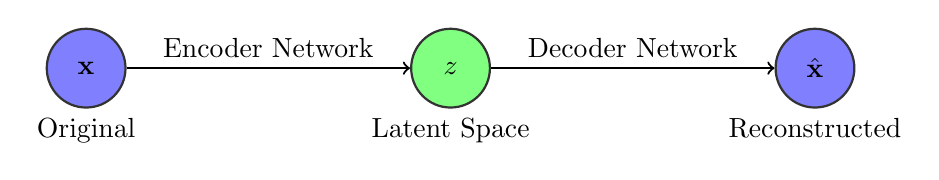
\begin{tikzpicture}
\tikzstyle{main}=[circle, minimum size = 10mm, thick, draw =black!80, node distance = 36mm]
\tikzstyle{connect}=[-latex, thick]
  \node[main, fill = blue!50] (alpha) [label=below: Original ] {$\x$};
  \node[main,fill = green!50] (z) [right=of alpha,label=below:Latent Space] { $z$};
  \node[main,fill = blue!50] (xout) [right= of z,label=below: Reconstructed ] {$\hat{\x}$ };
  \draw[thick,->] (alpha) -- (z) node[midway,sloped,above] {Encoder Network};
  \draw[thick,->] (z) -- (xout) node[midway,sloped,above] {Decoder Network};
  \end{tikzpicture}
  \caption{Loss function for a given input vector is usually their reconstruction error, i.e.,$\loss(\x)= ( \x-\hat{\x} )^2$}
\end{figure}

\end{frame}


\section{Autoencoder}
\begin{frame}{Autoencoder}
\begin{itemize}
\item An \emph{autoencoder} is a neural network that is trained to attempt to copy its input to its output.
\item The network may be viewed as consisting of two parts: an
encoder function $h = f (\X)$ and a decoder that produces a reconstruction $r(\X) = g(h(\X))$.
\item The composition of $f$ and $g$ is called the \emph{reconstruction function}
\item If an autoencoder succeeds to learn $g(f (\X)) = \X$ everywhere, then it is not especially useful (overfitting).
\item The learning process can be described as minimizing the loss function:
\begin{equation}
\loss ( \X , g(f(\X))),
\end{equation}
where $\loss$ is a loss function, such as mean squared error.
\end{itemize}
\begin{figure}
\centering
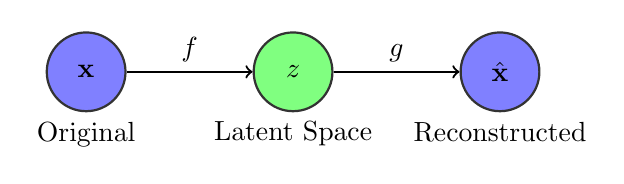
\begin{tikzpicture}
\tikzstyle{main}=[circle, minimum size = 10mm, thick, draw =black!80, node distance = 16mm]
\tikzstyle{connect}=[-latex, thick]
  \node[main, fill = blue!50] (alpha) [label=below: Original] {$\x$};
  \node[main,fill = green!50] (z) [right=of alpha,label=below:Latent Space] { $z$};
  \node[main,fill = blue!50] (xout) [right= of z,label=below: Reconstructed] {$\hat{\x}$ };
  \draw[thick,->] (alpha) -- (z) node[midway,sloped,above] {$f $};
  \draw[thick,->] (z) -- (xout) node[midway,sloped,above] {$g$};
  \end{tikzpicture}
  \caption{General Autoencoder structure}
\end{figure}
\end{frame}

\begin{frame}{Over/Under complete autoencoders}

\begin{figure}
\begin{tikzpicture}
\tikzstyle{main}=[circle, minimum size = 10mm, thick, draw =black!80, node distance = 6mm]
\tikzstyle{connect}=[-latex, thick]
  \node[main, fill = blue!50] (alpha) [label=below: $\mathbb{R}^\nfeatures$ ] {$\x$};
  \node[main,fill = green!50, scale=2] (z) [right=of alpha,label=below: $\mathbb{R}^K$] { $z$};
  \node[main,fill = blue!50] (xout) [right= of z,label=below: $\mathbb{R}^\nfeatures$] {$\hat{\x}$ };
  \draw[thick,->] (alpha) -- (z) node[midway,sloped,above] {$f$};
  \draw[thick,->] (z) -- (xout) node[midway,sloped,above] {$g$};
  \end{tikzpicture}
  \caption{$\nfeatures< K$: Overcomplete AE}
\end{figure}

\begin{figure}
\begin{tikzpicture}
\tikzstyle{main}=[circle, minimum size = 10mm, thick, draw =black!80, node distance = 6mm]
\tikzstyle{connect}=[-latex, thick]
  \node[main, fill = blue!50] (alpha) [label=below: $\mathbb{R}^\nfeatures$ ] {$\x$};
  \node[main,fill = green!50, scale=0.5] (z) [right=of alpha,label=below: $\mathbb{R}^K$] { $z$};
  \node[main,fill = blue!50] (xout) [right= of z,label=below: $\mathbb{R}^\nfeatures$] {$\hat{\x}$ };
  \draw[thick,->] (alpha) -- (z) node[midway,sloped,above] {$f$};
  \draw[thick,->] (z) -- (xout) node[midway,sloped,above] {$g$};
  \end{tikzpicture}
  \caption{$K < \nfeatures$: Undercomplete AE}
\end{figure}
An autoencoder whose code dimension is less than the input dimension is called \texttt{undercomplete}.
\end{frame}
%\begin{figure}
%\includegraphics[height=2.4cm]{../graphics/SallowUnderComplete}
%\includegraphics[height=2.4cm]{../graphics/DeepUnderComplete}\\
%\caption{(a)Sallow Under Complete (b)Deep Under Complete}
%\end{figure}
%\begin{figure}
%\includegraphics[height=2.4cm]{../graphics/SallowOverComplete}
%\includegraphics[height=2.4cm]{../graphics/DeepOverComplete}
%\caption{ (c)Sallow Over Complete (d)Deep Over Complete}
%\end{figure}

\subsection{Autoencoder}
\begin{frame}{Dimensional reduction methods}
When the decoder is linear and $\loss$ is the mean squared error, an undercomplete autoencoder learns to span the same subspace as PCA.
\begin{figure}
\includegraphics[width=.9\columnwidth]{../graphics/DimensionalityReduction}
\end{figure}
\end{frame}

\begin{frame}{Autoencoder vs general data compression methods}
\begin{itemize}
\item Autoencoder are data-dependent
\item MP3 or JPEG compression algorithm make general assumptions about "sound/images?, but not about
specific types of sounds/image.
\item Autoencoders are lossy.
\item Autoencoders are learnt for a specific application.
\end{itemize}
\end{frame}



\begin{frame}{Motivation: Nonlinear dimensionality reduction}
\begin{figure}
\includegraphics[width=.8\columnwidth]{../graphics/ManifoldLearning}
\caption{TODO: Manifold Learning}
\end{figure}
\end{frame}

\subsection{Type of Autoencoder}
\begin{frame}{Type of Autoencoders:}
\begin{enumerate}
\item Vanilla autoenconder
\item Regularized autoencoder (Sparse)
\item Denoising autoenconder
\item Contractive autoenconder
\item Variational autoenconder
%\item Stacked Autoencoders
\end{enumerate}
\end{frame}

\begin{frame}{Vanilla (Standard) Autoencoder}
\begin{figure}
\includegraphics[width=.8\columnwidth]{../graphics/StandardAutoencoder}
\caption{Vanilla Autoencoder.  Poor initialization can lead to local minima.}
\end{figure}
\begin{itemize}
\item Rumelhart, Hinton, Williams [RHW88]: Random Initialization and gradient descent shows bad performance.
\item Bengio, Lamblin, Popovici, Larochelle [BLP+07] [PCL06]: Stacking Autoencoders and tune with gradient descent shows good performance.
\end{itemize}
\end{frame}


\begin{frame}{Regularized Autoencoders}
A sparse autoencoder is simply an autoencoder whose training criterion involves a
sparsity penalty $\Omega(h)$ on the code layer $h$, in addition to the reconstruction error:
\begin{equation}
\loss ( \X , g(f(\X)))+\Omega(h)
\end{equation}
\begin{itemize}
\item $L_1$ : Cost function = Loss Function $+ \frac{\lambda}{2 m } \sum ||w||$
\item $L_2$  Cost function = Loss Function $+ \frac{\lambda}{2 m } \sum ||w||^2$
\end{itemize}
\begin{figure}
\includegraphics[width=.8\columnwidth]{../graphics/regularizers}
\caption{Regularizers in Keras. Note: Kernel and bias regularizer are not the same.}
\end{figure}
\end{frame}

\begin{frame}{Sparse Autoencoders}
Regularization of the representation learned by the Auto-Encoders.
\begin{itemize}
\item Enforcing most code coefficients to be close to 0 (to be inactive).
\item Capturing a more robust representation of the manifold structure.
\end{itemize}
Common implementation
\begin{itemize}
\item Adding a sparsity regularizer loss to the autoencoder loss function.
\item Various sparsity regularizers.
\item Other existing methods: 
\end{itemize}
\end{frame}


\begin{frame}{Contractive Autoencoders}
The \emph{contractive autoencoder} introduces a regularizer on the code $h = f(\X)$, encouraging the derivatives of $f$ to be as small as possible:
\begin{equation}
\Omega(h)=\lambda \left \lVert \frac{\partial f(\X)}{\partial \X} \right \lVert ^2_{F}
\end{equation}
TODO
\begin{figure}
\includegraphics[width=.5\columnwidth]{../graphics/Contractive}
\end{figure}
\end{frame}

\begin{frame}{Denoising Autoencoders (DAE)}
\begin{equation}
\loss ( \X , g(f(\tilde{\X}))),
\end{equation}
where $\tilde{\X}$ is a corrupted copy of $\X$ by some form of noise.
An overcomplete autoencoder with high capacity can end up learning an
identity function where input=output.
Add noise to

\begin{figure}
\begin{tikzpicture}
\tikzstyle{main}=[circle, minimum size = 10mm, thick, draw =black!80, node distance = 6mm]
\tikzstyle{connect}=[-latex, thick]
  \node[main, fill = blue!50] (alpha) [label=below: $\mathbb{R}^\nfeatures$ ] {$\x$};
  \node[main, fill = yellow!50] (Noise) [right=of alpha,label=below: Noise ] {$\epsilon$};
  \node[main,fill = green!50, scale=1] (z) [right=of Noise,label=below: $\mathbb{R}^K$] { $z$};
  \node[main,fill = blue!50] (xout) [right= of z,label=below: $\mathbb{R}^\nfeatures$] {$\hat{\x}$ };
  \draw[thick,->] (alpha) -- (Noise) node[midway,sloped,above] {$+$};
   \draw[thick,->] (Noise) -- (z) node[midway,sloped,above] {$f$};
  \draw[thick,->] (z) -- (xout) node[midway,sloped,above] {$g$};
  \end{tikzpicture}
\end{figure}
\end{frame}

\begin{frame}{Interpretation: Manifold Learning}
\begin{figure}
\includegraphics[width=.5\columnwidth]{../graphics/Manifold}
\end{figure}
\begin{itemize}
\item training data lies nearby a low-dimensional manifold.
\item a corrupted example is obtained by applying a perturbation of original example
\item The model should learn to \emph{project them back} to the manifold
\end{itemize}
TODO
\end{frame}


\begin{frame}{Modern Autoencoder}
\begin{itemize}
\item Modern autoencoders have generalized the idea of an encoder and a decoder
beyond deterministic functions to stochastic mappings
$p_{\texttt{encoder}}(h|\X)$ and $p_{\texttt{decoder}}(\X|h)$.
%\item 
%An autoencoder whose code dimension is less than the input dimension is called \texttt{undercomplete}. Goal: to capture the most salient features of the
%training data.
%\item
%The learning process can be described as minimizing the loss function:
%\begin{equation}
%\loss ( \X , g(f(\X))),
%\end{equation}
%where $\loss$ is a loss function, such as mean squared error.
%\item When the decoder is linear and $\loss$ is the mean squared error, an undercomplete
%autoencoder learns to span the same subspace as PCA.
\end{itemize}
\end{frame}

\begin{frame}{Variational Autoencoder}
\begin{figure}
\centering
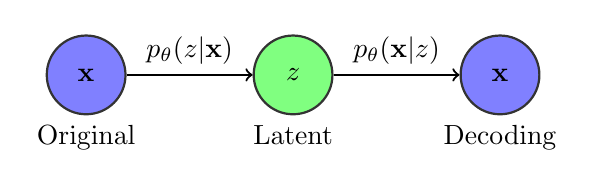
\begin{tikzpicture}
\tikzstyle{main}=[circle, minimum size = 10mm, thick, draw =black!80, node distance = 16mm]
\tikzstyle{connect}=[-latex, thick]
  \node[main, fill = blue!50] (alpha) [label=below:Original] {$\x$};
  \node[main,fill = green!50] (z) [right=of alpha,label=below:Latent] { $z$};
  \node[main,fill = blue!50] (xout) [right= of z,label=below: Decoding] {$\x$ };
  \draw[thick,->] (alpha) -- (z) node[midway,sloped,above] {$p_{\theta}(z|\x)$};
  \draw[thick,->] (z) -- (xout) node[midway,sloped,above] {$p_{\theta}(\x|z)$};
  \end{tikzpicture}
\end{figure}
\begin{itemize}
\item Training via maximum likelihood of $p(\x)$
\item Intractability: the true posterior density $p_{\theta}(z|\x)$ can be calculated %= p_{\theta}(\x|z)p_{\theta}(z)/p_{\theta}(\x)$ is intractable.
\item Solutions: a) MCMC (too costly) b) Approximate $p(z|\x)$ by means of $q(z|\x)=\mathcal{N}(z; \mu_{z}(x),\sigma_{z}(x))$
\end{itemize}
\end{frame}


\subsection{Variational Autoencoder}
\begin{frame}{Variational Autoencoder}
\begin{figure}
\centering
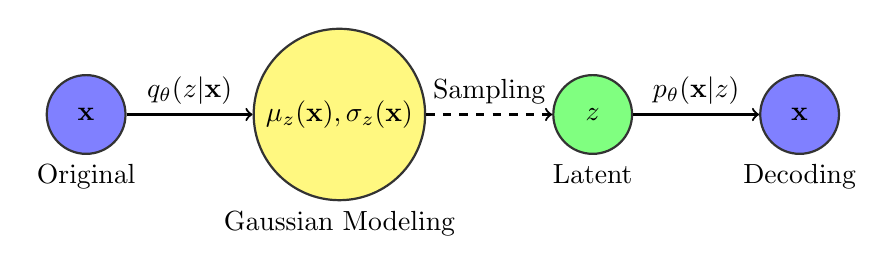
\begin{tikzpicture}
\tikzstyle{main}=[circle, minimum size = 10mm, thick, draw =black!80, node distance = 16mm]
\tikzstyle{connect}=[-latex, thick]
  \node[main, fill = blue!50] (alpha) [label=below:Original] {$\x$};
  \node[main,fill = yellow!50] (zsampling) [right=of alpha,label=below:Gaussian Modeling] { $\mu_{z}(\x),\sigma_{z}(\x)$};
  \node[main,fill = green!50] (z) [right=of zsampling,label=below:Latent] { $z$};
  \node[main,fill = blue!50] (xout) [right= of z,label=below: Decoding] {$\x$ };
  \draw[thick,->] (alpha) -- (zsampling) node[midway,sloped,above] {$q_{\theta}(z|\x)$};
  \draw[thick,->,dashed] (zsampling) -- (z) node[midway,sloped,above] {Sampling};
  \draw[thick,->] (z) -- (xout) node[midway,sloped,above] {$p_{\theta}(\x|z)$};
  \end{tikzpicture}
\end{figure}
\begin{itemize}
\item Gaussian modeling (diagonal covariance matrix to avoid problems in high dimensionality)
\item Training via maximum likelihood of $p(\x)$
\item Learning the parameters $\theta$'s via backpropagation?
%\item Loss function?
\end{itemize}
\end{frame}

\begin{frame}{Training via maximum likelihood}
Assume we would like to compute the likelihood of an image $\x$ from the training set:
\begin{eqnarray*}
\mathcal{L}(\x) &=&\log(p(\x)) \\
&=& \sum_{z} q(z|\x) \log(p(\x)) \\
&=& \sum_{z} q(z|\x) \log(\frac{p(z,\x)}{p(z | \x)}) \\
&=& \sum_{z} q(z|\x) \log(\frac{p(z,\x) q(z|\x)}{q(z|\x) p(z | \x)}) \\
&=&  \sum_{z} q(z|\x) \log(\frac{p(z,\x) }{q(z|\x)}) + \sum_{z} q(z|\x) \log(\frac{q(z|\x) }{p(z|\x)}) \\
&=& \sum_{z} q(z|\x) \log(\frac{p(z,\x) }{q(z|\x)})+ \underbrace{D_{KL}(q(z|\x),p(z|\x))}_{\text{how good is the approximation.}}\\
&=& \mathcal{L}^{lvb}(\x)+D_{KL}(q(z|\x),p(z|\x)) \\
&\geq& \mathcal{L}^{lvb}(\x)
\end{eqnarray*}
\end{frame}


\begin{frame}
$ \texttt{TODO CHECK}$
\begin{eqnarray*}
 \mathcal{L}(\x) \geq \mathcal{L}^{lvb}(\x) &=& \sum_{z} q(z|\x) \log(\frac{p(z,\x) }{q(z|\x)}) \\
 &=& \sum_{z} q(z|\x) \log(\frac{p(\x | z) p(z)}{q(z|\x)}) \\
 &=& \sum_{z} q(z|\x) \log(\frac{p(\x | z)}{q(z|\x)}) +  \sum_{z} q(z|\x) \log(\frac{p(z)}{q(z|\x)}) \\
 &=& \EV_{q(z|\x)} \log(p(\x | z)) -D_{KL}(q(z|\x),p(z))\\
  &=& \underbrace{\EV_{q(z|\x)} \log(p(\x | z))}_{\texttt{Expected Reconstruction}} - \underbrace{D_{KL}(q(z|\x),p(z))}_{\texttt{Regularization $\mathcal{N}(0,1)$}}\\
\end{eqnarray*}
\begin{itemize}
\item First term implies the use of many realization of sampling process (in practice we only a few of samples per training example!)
\item Second term is simply a formula for diagonal multivariate Gaussian distribution.
\end{itemize}
\end{frame}

\begin{frame}{Reparametrization trick}
Backpropagation is not possible through random sampling!
\begin{figure}
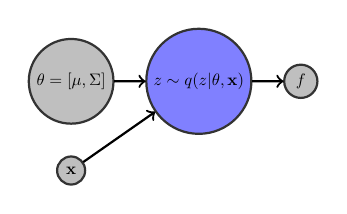
\begin{tikzpicture}[thick,scale=0.6, every node/.style={scale=0.6}]
\tikzstyle{main}=[circle, minimum size = 5mm, thick, draw =black!80, node distance = 4mm]
\tikzstyle{connect}=[-latex, thick]
  \node[main, fill = gray!50] (x) [] {$\x$};
   \node[main, fill = gray!50] (theta) [above=of x] {$\theta=[\mu,\Sigma]$};
   \node[main, fill = blue!50] (z) [right=of theta] {$z \sim q(z|\theta,\x)$};
   \node[main, fill = gray!50] (f) [right=of z] {$f$};
  %\node[main,fill = yellow!50] (zsampling) [right=of alpha,label=below:Gaussian Modeling] { $\mu_{z}(\x),\sigma_{z}(\x)$};
  %\node[main,fill = green!50] (z) [right=of zsampling,label=below:Latent] { $z$};
  %\node[main,fill = blue!50] (xout) [right= of z,label=below: Decoding] {$\x$ };
  \draw[thick,->] (x) -- (z) node[midway,sloped,above] {};
  \draw[thick,->] (theta) -- (z) node[midway,sloped,above] {};
  \draw[thick,->] (z) -- (f) node[midway,sloped,above] {};
  %\draw[thick,->,dashed] (zsampling) -- (z) node[midway,sloped,above] {Sampling};
  %\draw[thick,->] (z) -- (xout) node[midway,sloped,above] {$p_{\theta}(\x|z)$};
  \end{tikzpicture}
  \caption{Original Formulation}
\end{figure}
\pause
\begin{figure}
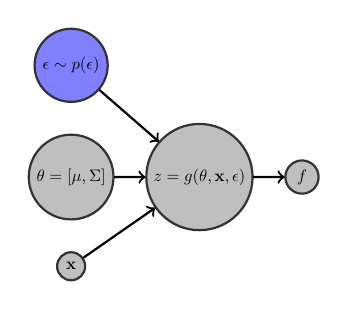
\begin{tikzpicture}[thick,scale=0.6, every node/.style={scale=0.6}]
\tikzstyle{main}=[circle, minimum size = 5mm, thick, draw =black!80, node distance = 4mm]
\tikzstyle{connect}=[-latex, thick]
  \node[main, fill = gray!50] (x) [] {$\x$};
   \node[main, fill = gray!50] (theta) [above=of x] {$\theta=[\mu,\Sigma]$};
   \node[main, fill = blue!50] (epsilon) [above=of theta] {$\epsilon \sim p(\epsilon)$};
   \node[main, fill = gray!50] (z) [right=of theta] {$z = g(\theta,\x,\epsilon)$};
   \node[main, fill = gray!50] (f) [right=of z] {$f$};
  %\node[main,fill = yellow!50] (zsampling) [right=of alpha,label=below:Gaussian Modeling] { $\mu_{z}(\x),\sigma_{z}(\x)$};
  %\node[main,fill = green!50] (z) [right=of zsampling,label=below:Latent] { $z$};
  %\node[main,fill = blue!50] (xout) [right= of z,label=below: Decoding] {$\x$ };
  \draw[thick,->] (x) -- (z) node[midway,sloped,above] {};
  \draw[thick,->] (theta) -- (z) node[midway,sloped,above] {};
   \draw[thick,->] (epsilon) -- (z) node[midway,sloped,above] {};
  \draw[thick,->] (z) -- (f) node[midway,sloped,above] {};
  %\draw[thick,->,dashed] (zsampling) -- (z) node[midway,sloped,above] {Sampling};
  %\draw[thick,->] (z) -- (xout) node[midway,sloped,above] {$p_{\theta}(\x|z)$};
  \end{tikzpicture}
  \caption{Reparametrization trick. Backpropagation}
\end{figure}
\end{frame}

\section{Applications for Autoencoders}

\begin{frame}
\begin{itemize}
\item Data denosing
\item Dimensionality Reduction
\item Database understanding
\item Generative models
\end{itemize}
\end{frame}


\begin{frame}{Example Latent Space for MNIST}
\begin{figure}
\includegraphics[width=.75\columnwidth]{../graphics/LatentMNIST}
\end{figure}
\end{frame}

%\begin{frame}{Galaxy Embedding}
%\begin{figure}
%\includegraphics[width=.5\columnwidth]{../graphics/GalaxyEmbedding}
%\caption{Jeffrey Regier et al, A deep generative model for astronomical images of galaxies}
%\end{figure}
%\end{frame}





\begin{frame}{Applications for Autoencoders}
\begin{enumerate}
\item Information retrieval using deep auto-encoders (semantic hashing)
\end{enumerate}
\end{frame}

\begin{frame}{KL-divergence between two multivariate Gaussian distributions}
\begin{eqnarray*}
KL(\mathcal{N}(\mu_0,\Sigma_0)) || \mathcal{N}(\mu_1,\Sigma_1))=\\
 \frac{1}{2} \left ( \tr (\Sigma_1^{-1}\Sigma_0)+(\mu_1-\mu_0)^T \Sigma_1^{-1}(\mu_1-\mu_0)-k+\log \left ( \frac{\det \Sigma_1}{\det \Sigma_0}\right )\right )
\end{eqnarray*}
where $k$ is the dimensionality of the distributions.
\end{frame}

\begin{frame}{Generative Adversarial Networks (GANs)}
\begin{figure}
\begin{tikzpicture}
\tikzstyle{main}=[circle, minimum size = 10mm, thick, draw =black!80, node distance = 9mm]
\tikzstyle{connect}=[-latex, thick]
  \node[main, fill = yellow!50] (Noise) [label=below: Noise ] {$\epsilon$};
   \node[main,fill = green!50, scale=1] (Generator) [right=of Noise, label=below: $G(z)$] { \texttt{Generator}};
  \node[main,fill = green!50] (Fake) [right= of Generator,label=below: Fake data] { $\hat{\x}$ };
    \node[main, fill = blue!50] (Data) [above=of Fake,label=below: $\mathbb{R}^\nfeatures$ ] {Real data $\x$};
   \node[main, fill = red!50] (Discriminator) [right=of Fake,label=below: $D(\x)$ ] {Discriminator};
  \node(Output) [text width=1cm] [right=of Discriminator]{1 real 0 fake};
  \draw[thick,->] (Data) -- (Discriminator) node[midway,sloped,above] {$P_{\texttt{real}}(\x)$};
   \draw[thick,->] (Noise) -- (Generator) node[midway,sloped,above] {$z$};
  \draw[thick,->] (Generator) -- (Fake) node[midway,sloped,above] {$P_z(z)$};
  \draw[thick,->] (Fake) -- (Discriminator) node[midway,sloped,above] {$$};
  \draw[thick,->] (Discriminator) -- (Output) node[midway,sloped,above] {$$};
  \end{tikzpicture}
\end{figure}
\pause
The goal is to optimize the follow expression, $\min_{G} \max _{D} V(D,G)$.
%for a given loss function $\loss(\cdot,\cdot)$.\\ 
\alert{We are looking the best generator for the best discriminator}.
\end{frame}

\begin{frame}{Generative Adversarial Networks (GANs)}
We require that the discriminator $D$ recognizes examples from the $P_{\texttt{real}}(\x)$ distribution,
\begin{equation*}
\mathbb{E}_{\x \sim P_{\texttt{real}}(\x)}[\log D(\x)]  \quad \quad \alert{\texttt{Decision over Real Data}}
\end{equation*} where $\mathbb{E}$ denotes the expectation. This term comes from the ``1" class  of the log-loss function. \\
Additionally, we would like to tricking the discriminator via a good generator $G$. Thus, the term comes from  ``0" class of the log-loss function:
\begin{equation*}
\mathbb{E}_{z \sim P_{z}(z)}[ \log (1-D(G(z)))]  \quad \quad  \alert{\texttt{Decision over Fake Data}}
\end{equation*}
\end{frame}

\begin{frame}{Optimal Discriminator? Optimal Generator?}
We define:
\begin{equation*}
V(G,D):= \mathbb{E}_{\x \sim P_{\texttt{real}}(\x)}[\log D(\x)] + \mathbb{E}_{z \sim P_{z}(z)}[ \log (1-D(G(z)))]
\end{equation*}
What should be an optimal discriminator? \pause
\begin{equation*}
D^* = \argmax_{D} V(G,D)
\end{equation*}
Now, given this optimal discriminator $D^*$, what should be an optimal generator? \pause
\begin{equation*}
G^* = \argmin_{G} V(G,D^*)
\end{equation*}
Minimax Game \cite{}
\end{frame}

\begin{frame}
\begin{eqnarray*}
&& \min_{G} \max _{D} V(D,G) := \\
&= &\mathbb{E}_{\x \sim P_{\texttt{real}}(\x)}[\log D(\x)]  + \mathbb{E}_{z \sim P_{z}(z)}[ \log (1-D(G(z)))]  \\
&&\texttt{by Radon-Nikodym Theorem} \\
&=& \mathbb{E}_{\x \sim P_{\texttt{real}}(\x)}[\log D(\x)]  + \mathbb{E}_{x \sim P_{\alert{{g}(\x)}}}[ \log (1-\alert{D(x)})]  
\end{eqnarray*}
An optimal generator should give $P_{g(\x)}=P_{\texttt{real}}(\x)$, and in this case:


\begin{equation}
\end{equation}
\end{frame}

\begin{frame}{Adversarial Example}
%For adversaries, an ideal adversarial attack is to construct a perturbed input $\x_{adv}$ with minimal distance to $\x$ to fool the DNN
%model, and yet its human user would still visually consider the adversarial input $\x_{adv}$ similar to or the same as the benign input $x$.
Given a benign sample $\x$, an adversarial example $\x_{adv}$ is generated by adding a small perturbation to $\x$ (i.e. $\x_{adv}=\x+\epsilon$), so that $\x_{adv}$ is misclassified by the targeted classifier $g$.

Formal definition:
(Adversarial example (Wang et al., 2016)). Given a ML model $f(\cdot)$ and \emph{a small perturbation $\delta$}, we call $\x_{adv}$ an adversarial example 
if there exists $x$, an example drawn from the benign data distribution, such that $f(\x)\neq f(\x_{adv})$ and $||\x - \x_{adv}|| \leq \delta$.
This is, $\x_{adv}$ could be called a \emph{counter example}.
\end{frame}

\begin{frame}
\begin{figure}
\includegraphics[width=.285\columnwidth]{../graphics/Adversarial0} \textbf{+}
\includegraphics[width=.285\columnwidth]{../graphics/Noise} \textbf{=}  
\includegraphics[width=.285\columnwidth]{../graphics/Adversarial2}
\caption{$\x$ + $\epsilon$ =  $\x_{adv}$}
\end{figure}

\begin{figure}
\includegraphics[width=.45\columnwidth]{../graphics/ClassX} 
\includegraphics[width=.45\columnwidth]{../graphics/ClassXadv} 
\caption{Prediction for: $\x$ and $\x_{adv}$}
\end{figure}
\end{frame}

%\begin{frame}
%\begin{figure}
%\includegraphics[width=.55\columnwidth]{../graphics/Adversarial2}
%\end{figure}
%From Explaining and Harnessing Adversarial Examples by Goodfellow et al.
%\end{frame}

%\begin{frame}
%\begin{figure}
%\includegraphics[width=.35\columnwidth]{../graphics/Noise}
%\end{figure}
%From Explaining and Harnessing Adversarial Examples by Goodfellow et al.
%\end{frame}

\begin{frame}{Adversarial Examples}
\textbf{Fast Gradient Sign Method}
Their perturbation can be expressed as
\begin{equation}
\eta =\epsilon sign(\nabla_{\x} J_{\param} (\x,\loss))
\end{equation}
where $\epsilon$ is the magnitude of the perturbation.
The generated adversarial example $\x'$ is calculated as $\x'=\x+\eta$.
This perturbation can be computed by using back-propagation.
\end{frame}

\begin{frame}{Universal Perturbation}
\begin{figure}
\includegraphics[width=.55\columnwidth]{../graphics/UniversalPerturbation}
\caption{ ?Universal adversarial perturbations}
\end{figure}
\end{frame}


%%%%%%%%%%%%%%%%%%%%%%%%%%%%%%%%%%%%%%%%%%%%%%%%%%
\section{References}
\begin{frame}
\begin{itemize}
\item Tutorial on Variational Autoencoders,CARL DOERSCH
\item http://jmlr.csail.mit.edu/papers/volume15/alain14a/alain14a.pdf
\item http://web.stanford.edu/class/cs294a/sae/sparseAutoencoderNotes.pdf
\item Contractive Auto-Encoders: Explicit Invariance During Feature Extraction.
Salah Rifai, Pascal Vincent, Xavier Muller, Xavier Glorot et Yoshua Bengio, 2011.
%https://arxiv.org/pdf/1606.05908.pdf
\end{itemize}
\end{frame}
%%%%%%%%%%%%%%%%%%%%%%%%%%%%%%%%%%%%%%%%%%%%%%%%%%


%%%%%%%%%%%%%%%%%%%%%%%%%%%%%%%%%%%%%%%%%%%%%%%%%%
%%%%%%%%%%%%%%%%%%%%%%%%%%%%%%%%%%%%%%%%%%%%%%%%%%
%%%%%%%%%%%%%%%%%%%%%%%%%%%%%%%%%%%%%%%%%%%%%%%%%%

\end{document}
